\documentclass[a4j,10pt]{jsarticle}
\usepackage{url}
\usepackage{proof}
% \usepackage{ascmac}
\usepackage[dvipdfmx]{graphicx}
% \usepackage[dvipdfmx]{color}
\pagestyle{plain}
\usepackage[dvipdfmx]{hyperref}
%\usepackage[textwidth=50zw,lines=51]{geometry}
\usepackage{amsthm}
\usepackage{amsmath, amssymb}
\usepackage{mathtools}
\mathtoolsset{showonlyrefs,showmanualtags}
% \mathtoolsset{showonlyrefs=true}
\usepackage{./resume}
\usepackage[dvipdfmx]{xcolor}% ドライバ指定のため
\usepackage{tikz}
\theoremstyle{definition}
\newtheorem{theorem}{定理}
\newtheorem*{theorem*}{定理}
\newtheorem{definition}{定義}
\newtheorem*{definition*}{定義}
\newtheorem{lemma}{補題}
\newtheorem*{lemma*}{補題}
\newtheorem{example}{例}
\newtheorem*{example*}{例}

\newcommand{\bnfdef}{::=}
\newlength{\len}
\settowidth{\len}{$\bnfdef$}
%\newcommand{\bnfor}{\makebox[\len]{$|$}}
\newcommand{\bnfor}{\mid}
\newcommand{\betah}{\longrightarrow_\beta }
\newcommand{\pbetah}{\Longrightarrow_\beta }
\newcommand{\alh}{\longrightarrow_\alpha}
\AtBeginDocument{
  \abovedisplayskip     =0.25\abovedisplayskip
  \abovedisplayshortskip=0.25\abovedisplayshortskip
  \belowdisplayskip     =0.25\belowdisplayskip
  \belowdisplayshortskip=0.25\belowdisplayshortskip}

\allowdisplaybreaks[1]

\title{Coqを用いたde Bruijn Indexにおける\\Church-Rosser Theoremの形式化}
\author{Arch B2 nem}

\begin{document}
\begin{abstract}
\(\lambda\)計算のnameless表現の1つである{\sl de Bruijn Index}について理解を深めるために\(\lambda\)計算の重要な性質である{\sl Church-Rosser}の定理をCoqを用いて{\sl de Bruijn Index}上で証明した.
\end{abstract}
\maketitle

\section{背景}
型理論への理解を深めることを目的に先学期から「型システム入門」\cite{tapl}をCoqで形式化\footnote{ここでいう形式化は定理証明支援系で証明を行うことを指す}をしていたが,{\sl de Bruijn Index}の関係で同じところで証明が詰まってしまっていたため,{\sl de Bruijn Index}の理解を深めること,自分の{\sl de Bruijn Index}の定義が正しいことを確認したいため期待している性質を{\sl de Bruijn Index}がもっていることを形式化した.\par
最初は名前による表現の\(\lambda\)計算\footnote{後述する一般的な\(\lambda\)計算のことを指す}と{\sl de Bruijn Index}の計算が等価であることを証明しようとした.命題は以下のものである.\par
{\sl de Bruijn Index}から名前による表現へ変換する関数を{\sl e}とし,名前による表現の\( \beta \)変換を\( \rightarrow_{name} \),{\sl de Bruijn Index}の\(\beta\)変換を\(\rightarrow_{dB}\)としたとき以下の命題が成り立つ.
\begin{align}
& M \rightarrow_{dB} N \Leftrightarrow e (M) \rightarrow_{name} e (N)
\end{align}
この命題について形式化を試みたとき,後述する捕獲回避代入(\ref{subst})など条件の多さから困難だった.\par
そこで,計算理論的な側面を形式化することにし,\(\lambda\)計算の重要な性質を表す{\sl Church-Rosser}の定理を形式化を行った.なお,名前による表現と{\sl de Bruijn Index}で共通の補題は高橋正子「計算論」\cite{takahashi}に,{\sl de Bruijn Index}特有の補題については{\sl "Fundamental Properties of Lambda-calculus"}\cite{isabelle}に基づいている. また,Coqのコードはgithubで公開している.\footnote{\href{https://github.com/NeM-T/ProofSandBox/blob/master/practice/coq/deBruijn/main.v}{https://github.com/nem-T/ProofSandBox/blob \\ /master/practice/coq/deBruijn/main.v}}

\section{定理証明支援系Coq}
定理証明支援系とは型理論及び数理論理学を基に計算機上で形式的な証明を行う環境を提供するソフトウェアのことを指す.\par
Coqは型理論の中でもCalculus of Inductive Constructions(CIC)を基にしている.\(\lambda\)計算におけるCICの推論規則は以下の規則である.なお,この規則は\cite{hal}に従っている.
\begin{definition*}
CICの推論規則
\begin{flalign}
& S \overset{\mathrm{def}}{=} \{Prop\} \cup \textstyle{\bigcup_{i \in \mathbb{N} }} \{Type_i\} \\
& \infer{\Gamma \vdash Prop: Type_1}{\Gamma \vdash}\\
& \infer{\Gamma \vdash Type_i: Type_{i + 1}}{\Gamma \vdash}\\
& \infer{\Gamma \vdash x: A}{\Gamma \vdash & x: A \in \Gamma}\\
& \infer{\Gamma, x: A \vdash }{\Gamma \vdash A: s & x \notin \Gamma & s \in S}\\
& \infer{\Gamma \vdash \lambda x: A.\, t: \Pi x: A.B }{\Gamma, x: A \vdash t: B}\\
& \infer{\Gamma \vdash f\ a: B[a\, /\, x]}{\Gamma \vdash f: \Pi x: A.B & \Gamma \vdash a: A}\\
& \infer{\Gamma \vdash \Pi x: A. B: Prop}{\Gamma, x: A \vdash B: Prop}\\
& \infer{\Gamma \vdash \Pi x: A.B: Type_u}{\Gamma, x: A \vdash B: Type_i & \Gamma \vdash A: Type_i}\\
& \infer{\Gamma \vdash t: B}{\Gamma \vdash t: A & \Gamma \vdash B: s & A \preceq B}
\end{flalign}
\par
$A \preceq B$はAがBよりちいさい{\sl Universe}である関係を表す。{\sl Universe}の大小関係は$Prop \preceq Type_1$,\, $Type_i \preceq Type_{i + 1}$で定義される。
\end{definition*}

\section{$\lambda$計算}
\(\lambda\)計算とは計算を引数の評価と適用によって表現した関数を形式的に扱うことのできる,チューリングマシン,帰納的関数と同等の計算能力をもつ計算モデルである.

\subsection* {\(\lambda\)式}
\begin{definition}
\(\lambda\)計算の式は以下によって再帰的に定義される.
\begin{itemize}
  \item xが変数ならばxは\(\lambda\)式である.
  \item xが変数,Mが\(\lambda\)式ならば$\lambda x. M$は\(\lambda\)式である.この形の式を$\lambda$抽象とよぶ.
  \item M, Nが\(\lambda\)式ならば$(M\, N)$は\(\lambda\)式である.この形の式を関数適用とよぶ.
  \item 以上によって定義されたもののみが\(\lambda\)式である.
\end{itemize}
\end{definition}

\subsection*{束縛}
$\lambda x. M$について\(M\) 内の変数xは束縛されていると表現し,xを束縛変数とよび,束縛されていない変数を自由変数とよぶ.形式的な定義は以下のようになる.
\begin{definition}
\(\lambda\)式\(M\) の自由変数の集合$FV (M)$
\begin{alignat}{2}
& FV (x) \ & = &\ \{x \} \\
& FV (\lambda x. M) \ & = &\  FV (M) \, \backslash\,  \{x\}\\
& FV (M\, N) \ & = &\  FV(M) \cup FV(N)
\end{alignat}
\end{definition}
\(\lambda\)式$M$が自由変数をもたない,($FV (M)\, =\, \emptyset$)とき\(M\) は閉じた\(\lambda\)式または閉式とよぶ.

\subsection*{$\alpha$変換}
ある束縛された変数をすべてある変数に置き換えたもの同士を$\alpha$同値性といい,置き換える操作を$\alpha$変換とよぶ.また,\(\lambda\)式{\sl M, N} について\( M \) を$\alpha$変換したものが\( N \) であることを$M \alh N$であらわす.\par
\begin{example*}
\begin{flalign}
& \lambda x.x \alh \lambda y.y\\
& \lambda x. (y (\lambda x. y\, x)x) \alh \lambda x. (y (/lambda z. y\, z)x)
\end{flalign}
\end{example*}

\subsection*{代入}
\(\lambda\)式\( M \) 内の自由変数xを\(\lambda\)式\(N\)に置き換える操作を代入とよび,$M [x:= N]$で表す.
\begin{definition}
代入
\begin{alignat}{2}
& x[x:=N] &\equiv\ & N\\
& y[x:=N] &\equiv\ & y \hspace{20pt} (x \neq y)\\
& (M_1\, M_2)[x:= N] &\equiv\ & (M_1[x:= N]\, M_2[x:= N])\\
& (\lambda x. M)[x:= N] &\equiv\ & \lambda x.M\\
& (\lambda y. M)[x:= N] &\equiv\ & \lambda y. (M[x:= N]) \notag \\
& & & (x \neq y,\, y \notin FV(N)) \label{eq:fvneed}
\end{alignat}
\end{definition}
\begin{example*}
\begin{align}
((\lambda x. y\, x)y)[y:= (\lambda z.z)] \equiv (\lambda x. (\lambda z. z) x)(\lambda z. z)
\end{align}
\end{example*}
\subsection*{捕獲回避代入}\label{subst}
\eqref{eq:fvneed} に条件$y \notin FV(N)$を課さない場合を考える.このとき,$(\lambda y. (x\, z))[x:= y] $を計算すると$\lambda y. y\, z$となり束縛関係が変わる.このような代入を変数の衝突といい,$y \notin FV(N)$を条件に加えることで回避している.\par
$y \in FV(N)$であるとき,代入する前に$\alpha$変換を行うことで変数の衝突を避けることが可能である.この操作を以下の定義を追加することで形式化できる.\par
\begin{alignat}{2}
    & (\lambda y. M)[x := N] \equiv \lambda z. M[y := z][x:= t]\\
    & \hspace{12pt} (x \neq y,\, y \in FV(N),\, z \notin {x} \cup FV(t)\cup FV(u))\\
\end{alignat}
このような代入を捕獲回避代入とよぶ.名前表現の\(\lambda\)計算を形式化をする際には捕獲回避代入を用いるが,\(\alpha\)同値性を明示的に証明を行う必要があるため,場合分けが多くなり複雑な証明になることから今回は{\sl de Bruijn Index}を使用した.\par
これ以降,代入の定義は捕獲回避代入を含んだ定義であるものとする.

\subsection*{$\beta$変換}
\(\lambda\)式内の$(\lambda x.M)\, N$を$M[x := N]$に置き換え,計算する操作を$\beta$変換とよぶ. \( M \) を$\beta$変換した結果が\(N\) であることを$M \betah N$と表記する.このとき計算規則は以下のように定義できる.
\begin{definition}
$\beta$変換の計算規則
\begin{alignat}{4}
& ((\lambda x. M) N)& &\betah\ & &M[x:= N]&\\
& \lambda x. M_1& &\betah\ & &\lambda x. M_2& &(M_1 \betah M_2)\\
& (M_1\, N)& &\betah\ & &(M_2\, N)& &(M_1 \betah M_2)\\
& (M\, N_1)& &\betah\ & &(M\, N_2)& &(N_1 \betah N_2)
\end{alignat}
\end{definition}
$(\lambda x. N)\, M$を$\beta$基とよび$\beta$基を含まない,すなわちそれ以上$\beta$変換できない形の\(\lambda\)式を$\beta$正規形($\beta${\sl -normal-form})とよぶ.
\begin{example*}
\begin{flalign}
& (\lambda x. x)y \betah y\\
& (\lambda x. x\, y)(\lambda x. x) \betah (\lambda x. x\, y)
\end{flalign}
\end{example*}

\subsubsection*{簡約の方法}
$\beta$変換は非決定的である. どの$\beta$基から簡約していくかは計算する側に委ねられている.以下に\(\lambda\)計算の主な計算戦略を記す.\par
\(\lambda\)式の内の$\beta$基の最も左にあるものから簡約していく操作を最左$\beta$変換,右を最右$\beta$変換とよぶ.\par
$(\lambda x. M)N$について\(N\) を計算した後に簡約する計算戦略を値呼び戦略,\(N\) を計算せずに簡約する戦略を名前呼び戦略とよぶ.\par

\subsubsection* {$\beta$変換列}
有限回の$\beta$変換で$M$から$N$へ到達するとき,すなわち以下を満たす$P_1, P_2, ..., P_n$が存在するとき,この列を$\beta$変換列といい,$M \twoheadrightarrow_\beta N$とかく.\par
\fbox{$M = P_1 \betah P_2 \betah \cdots P_n = N$}

\section{\sl \textbf{de Bruijn Index}}
変数の表現方法が変数名ではなく,内側から数えた束縛位置を表す自然数となっている\(\lambda\)式の表現方法において自由変数を(与えられたリストの位置+深さ)で表したものを{\sl de Bruijn Index}とよぶ.自由変数は名前による表現を用いるものもあり,そちらは{\sl Locally Nameless}表現とよぶ.
\begin{example*}
自由変数のリストは[a, b]とする.
\begin{align}
& \lambda x. x \equiv \lambda. 0\\
& \lambda f. (\lambda x. f (\lambda y. (x\, x)\, y)) \equiv \lambda . (\lambda. 1\, (\lambda . (1\, 1)\, 0))\\
& \lambda x. (a\, (\lambda y. (x\, b))) \equiv \lambda .(1\, (\lambda. (1\, 3)))
\end{align}
\end{example*}

\subsection*{\sl \textbf{de Bruijn Indexの代入}}
{\sl de Bruijn Index}の代入において\(\lambda\)抽象に対して代入をする際に,代入される\(\lambda\)式と深さを等しくするために代入する\(\lambda\)式の深さを変更するシフト関数が必要となる.
\begin{definition}
シフト関数\(\uparrow\)
\begin{alignat}{2}
    & x \uparrow_c^d & =\ & \left\{ 
    \begin{array}{ll}
         x + d & (c \leq x) \\
         x & (x < c)
    \end{array} \right. \\
    & (M\, N)\uparrow_c^d & =\ & (M \uparrow_c^d\, N \uparrow_c^d)\\
    & (\lambda . M)\uparrow_c^d & =\ &\lambda. (M \uparrow_{c+1}^d)\\
    & M \uparrow^d & =\ & M\uparrow_0^d
\end{alignat}
\end{definition}
このとき,自然な{\sl de Bruijn Index}の代入と\(\beta\)変換の定義は以下のものである.
\begin{definition}
代入の定義(1)
\begin{alignat}{2}
    & y[x:=N] &=\ & \left\{
    \begin{array}{ll}
        N &(x = y) \\
        y & (x \neq y) 
    \end{array} \right. \\
    & (M_1\, M_2)[x:=N] &=\ & (M_1[x:=N]\, M_2[x:=N]) \\
    & (\lambda. M)[x:= N] &=\ & \lambda. (M[x + 1 := N\uparrow^1])
\end{alignat}
\end{definition}
\begin{definition}
\(\beta\)変換の定義(1)
\begin{align}
    ((\lambda. M) N) &\betah& &M[0:= (N \uparrow^1) ]\uparrow^{-1} \\
    \lambda. M_1 &\betah& &\lambda x. M_2 \hspace{20pt} (M_1 \betah M_2)\\
    (M_1\, N) &\betah& &(M_2\, N) \hspace{20pt} (M_1 \betah M_2)\\
    (M\, N_1) &\betah& &(M\, N_2) \hspace{20pt} (N_1 \betah N_2)
\end{align}
\end{definition}
上の定義には\(\uparrow^{-1}\)を含んでおり,このことが形式化を困難にしている.そこで,\(\beta\)変換に使うことを前提として,代入の段階で処理をしてしまう定義が以下のものである.
\begin{definition}
代入の定義(2)
\begin{alignat}{4}
    & y[x:=N]& &=\ & & \left\{
    \begin{array}{lll}
        y - 1 & (x < y)\\
        N &(x = y) \\
        y & (y > x) 
    \end{array} \right. &\\
    & (M_1\, M_2)[x:=N]& &=\ & &(M_1[x:=N]\, M_2[x:=N])& \\
    & (\lambda. M)[x:= N]& &=\ & &\lambda. (M[x + 1 := N\uparrow^1])&
\end{alignat}
\end{definition}
\begin{definition}
\(\beta\)変換の定義(2)
\begin{align}
    ((\lambda. M) N) &\betah& & M[0:= N] & \\
    \lambda. M_1 &\betah& &\lambda x. M_2 &(M_1 \betah M_2)\\
    (M_1\, N) &\betah& &(M_2\, N) & (M_1 \betah M_2)\\
    (M\, N_1) &\betah& &(M\, N_2) & (N_1 \betah N_2)
\end{align}
\end{definition}
今回使用した定義は(2)であるが代入の定義には\ \(t\uparrow^1 \cdots n \cdots\uparrow^1 = t \uparrow^n\)\ であることを利用して\(\lambda\)抽象のシフトをひとまとめにする定義が存在する.その定義は以下のものである.
\begin{definition}
代入の定義(3)
\begin{alignat}{4}
    & y[x:=N]& &=\ & &\left\{
    \begin{array}{lll}
        y - 1 & (x < y)\\
        N\uparrow^x &(x = y) \\
        y & (y > x) 
    \end{array} \right. &\\
    & (M_1\, M_2)[x:=N]& &=\ & & (M_1[x:=N]\, M_2[x:=N])& \\
    & (\lambda. M)[x:= N]& &=\ & & \lambda. (M[x + 1 := N])&
\end{alignat}
\end{definition}


\section{\sl \textbf{Church-Rosser Theorem}}

\begin{theorem}
{\sl Church-Rosserの定理}\par
$M \twoheadrightarrow M_1,\, M \twoheadrightarrow M_2 \mbox{ならば} M_1 \twoheadrightarrow N \land M_2 \twoheadrightarrow N$を満たす$N$が存在する.
\end{theorem}
{\sl Church-Rosser}の定理はある\(\lambda\)式$M$から「$\twoheadrightarrow_\beta$」で得られた\(\lambda\)式はすべてある\(\lambda\)式$N$に「$\twoheadrightarrow_\beta$」で合流することを意味している.\par
{\sl Church-Rosser}の定理が成り立つことで以下の定理が成り立つ.
\begin{theorem}
正規化定理\par
任意の\(\lambda\)式$M$が正規形$N$をもつならば有限回の最左$\beta$変換で$N$に到達することが可能である.
\end{theorem}

\subsection*{証明の指針}
{\sl Church-Rosser}は以下の命題が成り立たないため, \(\betah\)と\(\twoheadrightarrow_\beta\)だけで証明するには複雑な証明になる.\vspace{7pt}\\
\(M \betah M_1, M \betah M_2\)ならば,\(M_1 \betah N \land M_2 \betah N\)を満たす\(\lambda\)式\(N\)が存在する.\vspace{7pt}\par
そのため,以下の性質をもつ新たな関係\(\pbetah\)が必要である.
\begin{align}
& M \pbetah N \hspace{20pt}(M \betah N) \label{one} \\
& M \twoheadrightarrow_\beta N \hspace{20pt} (M \pbetah N)\label{two} \\
& M_1 \pbetah N \land M_2 \pbetah N\\ 
    &  \hspace{20pt} (M \pbetah M_1 \land M \pbetah M_2)\label{three}
\end{align}

\eqref{one},\eqref{two}から\(M \twoheadrightarrow_\beta N\)と有限回の\(\pbetah\)で\(M\)から\(N\)に到達できることが同値であることを表している.\\
有限回の\(\pbetah\)で\(M\)から\(N\)へ到達することが可能であることを\(M \Longrightarrow_\beta\ast\, N\)と表すとき,\eqref{three}から以下の命題が成り立つ.
\begin{lemma*}
\begin{align}
 M_1 \Longrightarrow_\beta\ast N &\land M_2 \Longrightarrow_\beta\ast N \\
 &(M \pbetah M_1 \land M \Longrightarrow_\beta\ast M_2)\label{ho}
\end{align}
\end{lemma*}
この補題から\eqref{one},\eqref{two},\eqref{three}を満たす関係\(\pbetah\)が存在したとき,{\sl Church-Rosser}の定理は成り立つ.

\subsection*{並列\(\beta\)変換}
上記の条件を満たす関係\(\pbetah\)に並列\(\beta\)変換がある.
\begin{definition*}
並列\(\beta\)変換の計算規則
\begin{alignat}{3}
& x &\pbetah\ & x\\
& \lambda . M &\pbetah\ &\lambda. N &(M \pbetah N)\\
& M_1\, N_1 &\pbetah\ & M_2\, N_2 \notag \\
    &&&(M_1 \pbetah M_2,& N_1 \pbetah N_2)\\
& (\lambda. M_1) N_1 &\pbetah\ & M_2[0:= N_2]& \notag\\
    & & &(M_1 \pbetah M_2,& N_1 \pbetah N_2)
\end{alignat}
\end{definition*}

\subsection*{補題}
\begin{lemma}
シフト,代入の性質
\begin{alignat}{3}
    & i < k + 1 \Longrightarrow (t\uparrow_i^1)\uparrow_{k + 1}^1= (t \uparrow_k^1)\uparrow_i^1\label{eq:shift-shift} \\
    & j < i + 1 \Longrightarrow (t[j:= s])\uparrow_i^1 = (t\uparrow_{i+1}^1)[j := s\uparrow_i^1]\label{eq:sub-shift} \\
    & j < i + 1 \Longrightarrow  (t[i := s]\uparrow_j^1)= (t \uparrow_j^1)[(i+1) := s\uparrow_j^1] \label{eq:sub-shift-lt}\\
    & (t\uparrow_k^1)[k := s] = t\label{shift-sub} \\
    & i < j + 1 \Longrightarrow t[(j + 1) := (v \uparrow_i^1)][i := (u [j := v])] \notag \\
    & \hspace{90pt} = t[i := u][j := v]\label{eq:subsub}
\end{alignat}
\end{lemma}

\begin{lemma}
並行\(\beta\)変換の補題
\begin{alignat}{3}
M &\pbetah & &M \label{eq:refl} \\
M \uparrow_n^1 &\pbetah & &N\uparrow_n^1 \hspace{3pt}(M \pbetah N) \label{eq:shif-pre} \\
M_1[x:= N_1] &\pbetah & &M_2 [x:= N_2]\\
&&& \hspace{-20pt}(M_1 \pbetah M_2, N_1 \pbetah N_2) \label{eq:sub-pre}
\end{alignat}
\end{lemma}

\subsubsection*{補題の依存関係}
\begin{center}
\begin{tikzpicture}
    \draw [->](0.25,12)--(1.75,12);
    \draw [->](0,11.75)--(0,10.25);
    \draw [->](0.25,11.75)--(1.75,10.25);
    \draw [->](2,11.75)--(2,10.25);
    \draw [->](0,9.75)--(0,8.25);
    \draw [->](2,9.75)--(2,8.25);
    \draw [->](0.35,8)--(1.65,8);
    \draw [->](2,7.75)--(2,6.25);
    \draw [->](1.75,6)--(0.25,6);
    \draw [->](0,5.75)--(0,4.25);
    \draw [->](2.75,4)--(1.25,4);
    \draw [->](3,5.75)--(3,4.25);
    \draw [->](-1.75,4)--(-1.25,4);
    \draw [->](2.75,10)--(2.35,10);
    \draw (0,12)node{\eqref{eq:shift-shift}};
    \draw (2,12)node{\eqref{eq:sub-shift-lt}};
    \draw (0,10)node{\eqref{eq:sub-shift}};
    \draw (3,10)node{\eqref{shift-sub}};
    \draw (2,10)node{\eqref{eq:subsub}};
    \draw (0,8)node{\eqref{eq:shif-pre}};
    \draw (2,8)node{\eqref{eq:sub-pre}};
    \draw (2,6)node{\eqref{three}};
    \draw (0,6)node{\eqref{ho}};
    \draw (0,4)node{\sl Church-Rosser};
    \draw (3,4)node{\eqref{one}};
    \draw (3,6)node{\eqref{eq:refl}};
    \draw (-2,4)node{\eqref{two}};
\end{tikzpicture}
\end{center}


\section{{$\lambda$}計算の簡易インタプリタの実装}
証明した評価器を用いて簡易的な\(\lambda\)計算のインタプリタを実装した.
\subsection*{開発環境}
CoqのCore LanguageであるGallinaで記述された関数,型はExtractionとよばれる機能を使用することでOCaml又はHaskellに変換可能である.今回はOCamlがCoqの文法に近いことからOCamlを用いて実装した. また,実装には字句解析器生成器ocamllex,構文解析器生成器Menhir,ビルドシステムDuneを使用した. 

\begin{figure}[htbp]
    \begin{center}
        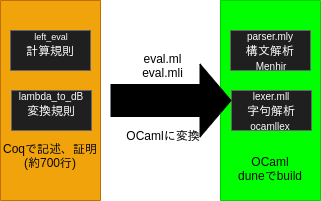
\includegraphics[width=6cm]{wip.png}
        \caption{構成}
        \label{sampleLaTeX Workshop}
    \end{center}
\end{figure}

\subsection*{実行}
実行手順は以下のようになっている.
\begin{enumerate}
    \item 名前表現の\(\lambda\)式で受け取る
    \item {\sl de Bruijn Index}に変換する
    \item {\sl de Bruijn Index}で最左\(\beta\)変換
    \item 名前表現の\(\lambda\)式に変換,出力
\end{enumerate}
名前表現の\(\lambda\)式を{\sl de Bruijn Index}に変換する関数を{\sl n\_to\_d},逆変換を{\sl d\_to\_n}としたとき,変換する関数については以下の命題を証明している.\vspace{7pt}
\begin{alignat}{3}
    &n\_to\_d (d\_to\_n\ t)& &=\ & t&\\
    &d\_to\_n (n\_to\_d\ t)& &=\ & t&
\end{alignat}

\section{まとめ}
目標とした{\sl Church-Rosser}の定理の形式化及び{\sl de Bruijn Index}の理解を達成することができた.
また,シフトと代入の補題を用いることで「型システム入門」の形式化で詰まっていた箇所の形式化を進めることができはじめた.
一方で,背景にも書いたが,名前表現と{\sl de Bruijn Index}との対応関係の形式化はできなかった.

\section{今後}
来学期中に型推論器の形式化を終えることを目標に「型システム入門」の形式化を進める予定である.
また,CICとZFCとの関係についての理解が浅いのでしっかり理解したい.
加えて,Coq,AgdaやIsabelle等証明支援系を比較した上で今後形式化を行うものを決めたい.

\nocite{*}
\bibliography{article}
\bibliographystyle{junsrt}

\end{document}
